Error-resilience is typically a topic discussed orthogonally to congestion
control and the main reason is that, error-resilience caters to handling
packet loss while congestion control caters to the amount of information sent
over the network. This chapter is based on our work on unifying
error-resilience and congestion control.

In \citepub{c:err}, we evaluate the performance of the various
error-resilience schemes available for use in interactive multimedia
communication (mainly applicable to H.264). These are: using Negative
Acknowledgement (NACK) or Packet Loss Indication (PLI), Forward Error
Correction (FEC) or Unequal Level of Protection (ULP), slice size adaption
(SSA), and Reference Pictures Selection Indication (RPSI). We evaluate the
performance of the proposed mechanisms in diverse scenarios in a simulated
environment (in ns-2) using real-world 3G loss patterns~\cite{3gppSim}.
Lastly, based on our observations, we define the applicability of the various
error-resilience with respect to end-to-end delay and packet loss.

In \citepub{c:fecrc}, we propose using FEC not only for error-resilience but
also for congestion control. Instead of probing for available capacity by
increasing the sending rate of the media flow, we propose introducing
redundancy. If a packet gets lost and the added FEC packet arrives in time the
receiving endpoint would recover the lost packet. However, if the packet is
not lost, by introducing the FEC packet the sender not only discovers that
there is additional available capacity, but also has a sense of the magnitude
(at minimum) of the available capacity. We compare our proposal with our
previous work in \citepub{c:3grc} and \citepub{c:hetrc}, and Google's
congestion control~\cite{draft.rrtcc}. We evaluate the performance of the
mechanisms in diverse scenarios implemented in a simulation environment (in
ns-2) and in our testbed.

\section{Error-resilience Schemes}
% explain all 4 and the adaptivity

H.264~\cite{h264} uses various error-control methods~\cite{err_res_h264_std,
wang98error, wang00review, 310669} to overcome loss due to bit-error
corruption (e.g., in wireless) and non-bursty packet loss (e.g., due to
congestion). These methods are classified into three categories: source
coding, channel coding, and joint source and channel methods. Source coding
refers to the methods implemented by the video codec. Channel coding refers to
the methods implemented by the networking layer. Joint source-channel refers
to methods that combine source-coding and network-coding mechanisms.

The H.264/AVC codec has several features that support error resilient
mechanisms for video communication that correspond to the above
categorization~\cite{310669}. At the codec level, the following are available:
Slice Size Adaptation (SSA), Reference Picture Selection (RPS), and Flexible
Macroblock Ordering (FMO)~\cite{err_res_h264_std, wenger_ott_jscc}. Similarly,
at the channel level, the following are available: Selective Retransmission
(NACK), Packet Loss Indication (PLI). An example of joint source-channel is
Unequal Error Protection (UEP) with FEC~\cite{wang00review}, the sender
attempts to selectively protect important parts of the bitstream or by
encoding redundant pictures differently than other pictures \cite{ervcuupkp}.

The performance of the available error-resilience mechanisms vary with the
observed end-to-end delay, link loss, bandwidth constraints and operating
environment (3G/LTE to 3G/LTE, 3G/LTE to WLAN, or wireless to fixed, etc.). No
single error repair mechanism fits all operating environments. A solution that
works for an observed packet loss ratio of less than 2\%, may not scale well
for paths with higher packet loss or higher latency.

% The combination of end-to-end delay requirements, capacity constraints and
% varying packet loss rate require different error resilience mechanisms.

\begin{figure}
\centerline {
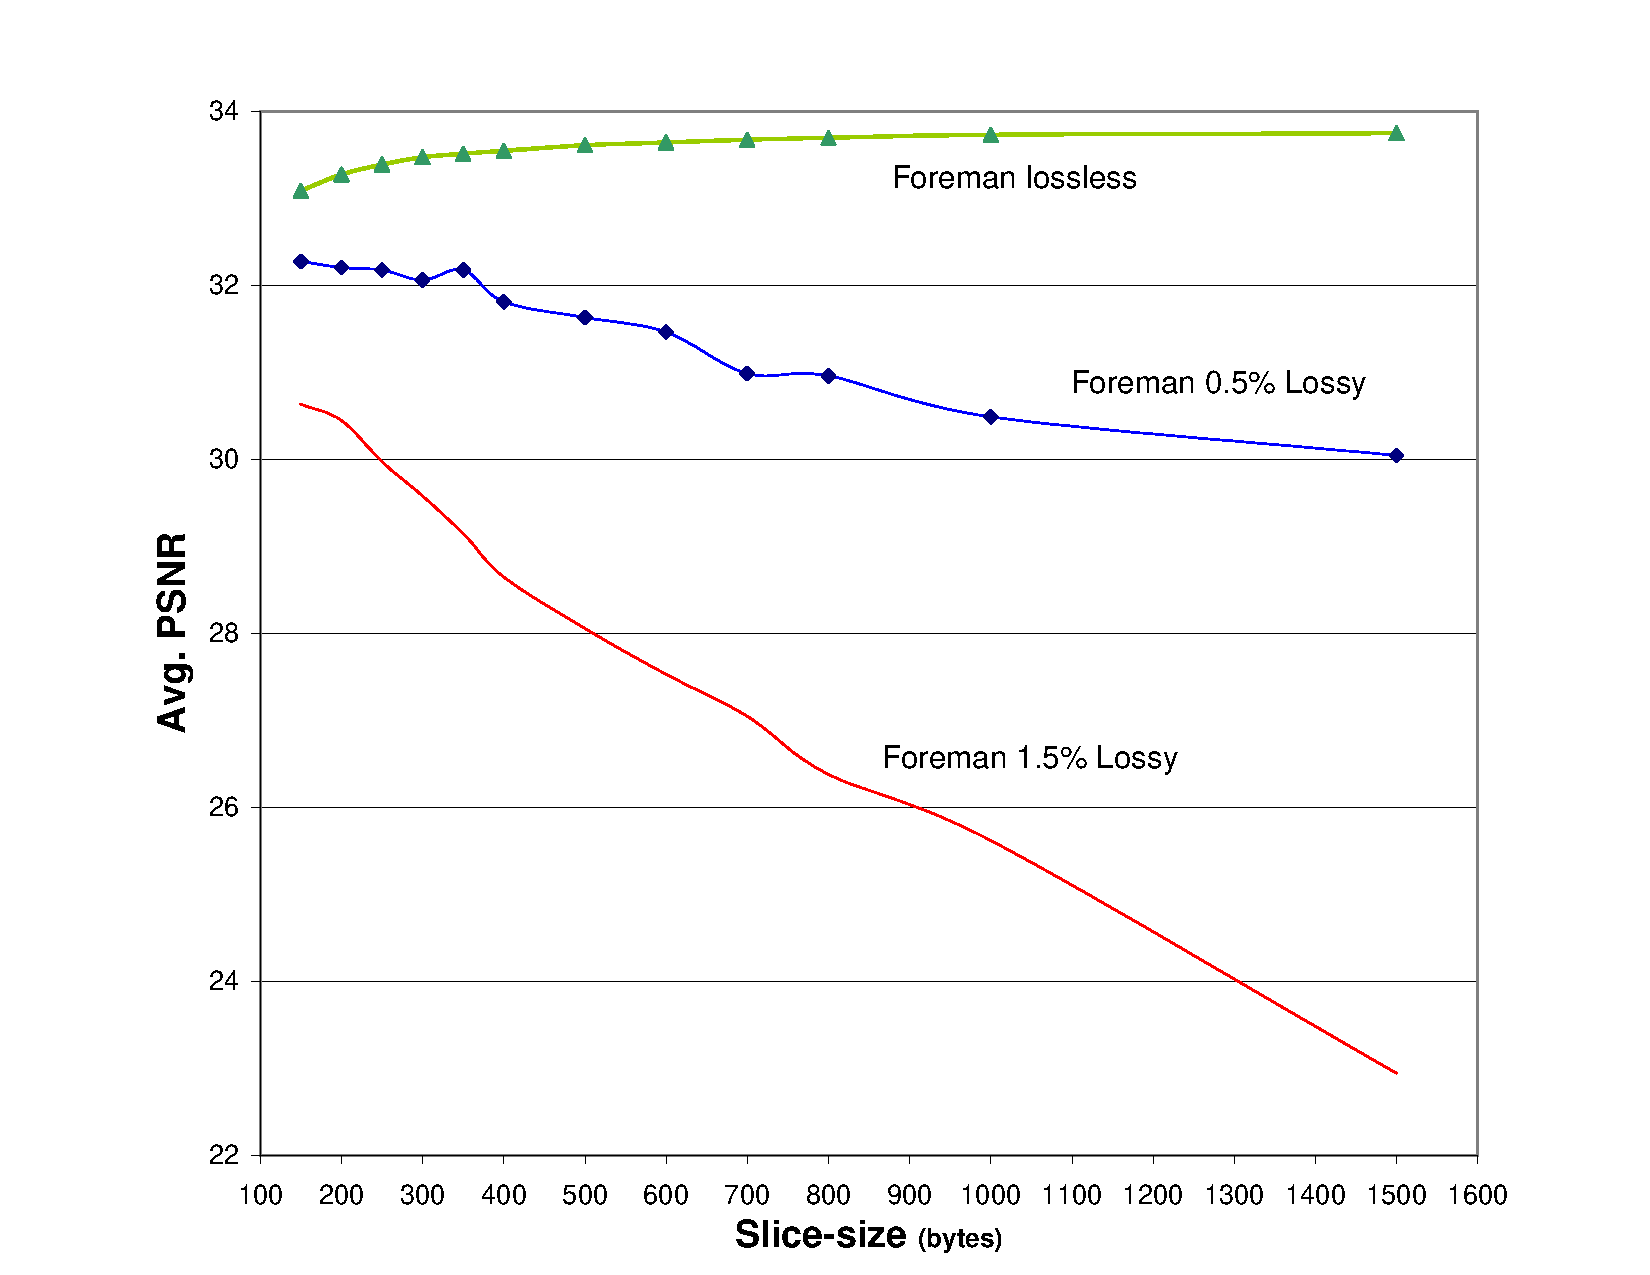
\includegraphics[width=0.75\textwidth]{chap6_slicesize_mot}
}
\caption{Effect of different slice sizes on PSNR for links observing bit-error
corruption.}
\label{fig:slicesize_mot}
\end{figure}

\begin{itemize}
\setlength{\itemsep}{0pt}

  \item \textbf{\texttt{Retransmissions}}: In RTP, retransmissions are either
  payload-specific or at the transport-specific. Transport-specific loss
  contains packet loss information (Generic NACK), while payload-specific loss
  contains Slice Loss Information (SLI), Picture Loss Information (PLI) or
  Reference Picture Selection indication (RPS). Typically, the receiver
  detects a loss and sends it as soon as the RTCP reporting interval allows
  feedback.

  \item \textbf{\texttt{Adapting Slice Sizes}}: the encoder adapts the size of
  the picture slice based on the link characteristics; when the channel is
  lossless there can be one picture per slice or be the MTU size and when the
  high losses are reported, the slices are reduced in size (up to 100 bytes).
  Larger slice sizes improve encoding efficiency, but are more vulnerable to
  frame losses. Figure~\ref{fig:slicesize_mot} shows the variation of average
  PSNR with respect to different slice-sizes in varying loss scenarios. We
  observe, that there is direct correlation between packet loss and slice
  size.

  \item \textbf{\texttt{Reference Picture Selection}}: Instead of
  retransmitting the lost packet, the encoder finds the list of correctly
  received pictures by the decoder. Hence, for subsequent encodings, the
  encoder uses a different decoded picture for inter prediction reference.
  This method stops the temporal error propagation caused by an earlier packet
  loss. In the RPS message, the decoder either reports the list of pictures
  that were correctly received or lost. Hence, the encoder is able to retrieve
  the required picture loss data. The mode of operation can be decided
  depending on the observed packet loss rate.

  \item \textbf{\texttt{Unequal Error Protection}}: When the link latency is
  high, retransmissions cannot be used. In high latency networks, the
  retransmitted packets arrive too late to be played back. In these cases, the
  sender proactively uses a portion of the available capacity to send
  redundant packets (typically, FEC), hoping to recover any lost packet before
  decoding. Hence, by using UEP, the media senders try to strike a balance by
  protecting only a chosen set of the media packets. In \cite{c:err}, we
  mainly protect reference frames with UEP.

\end{itemize}


% \begin{figure}
% \centerline {
% 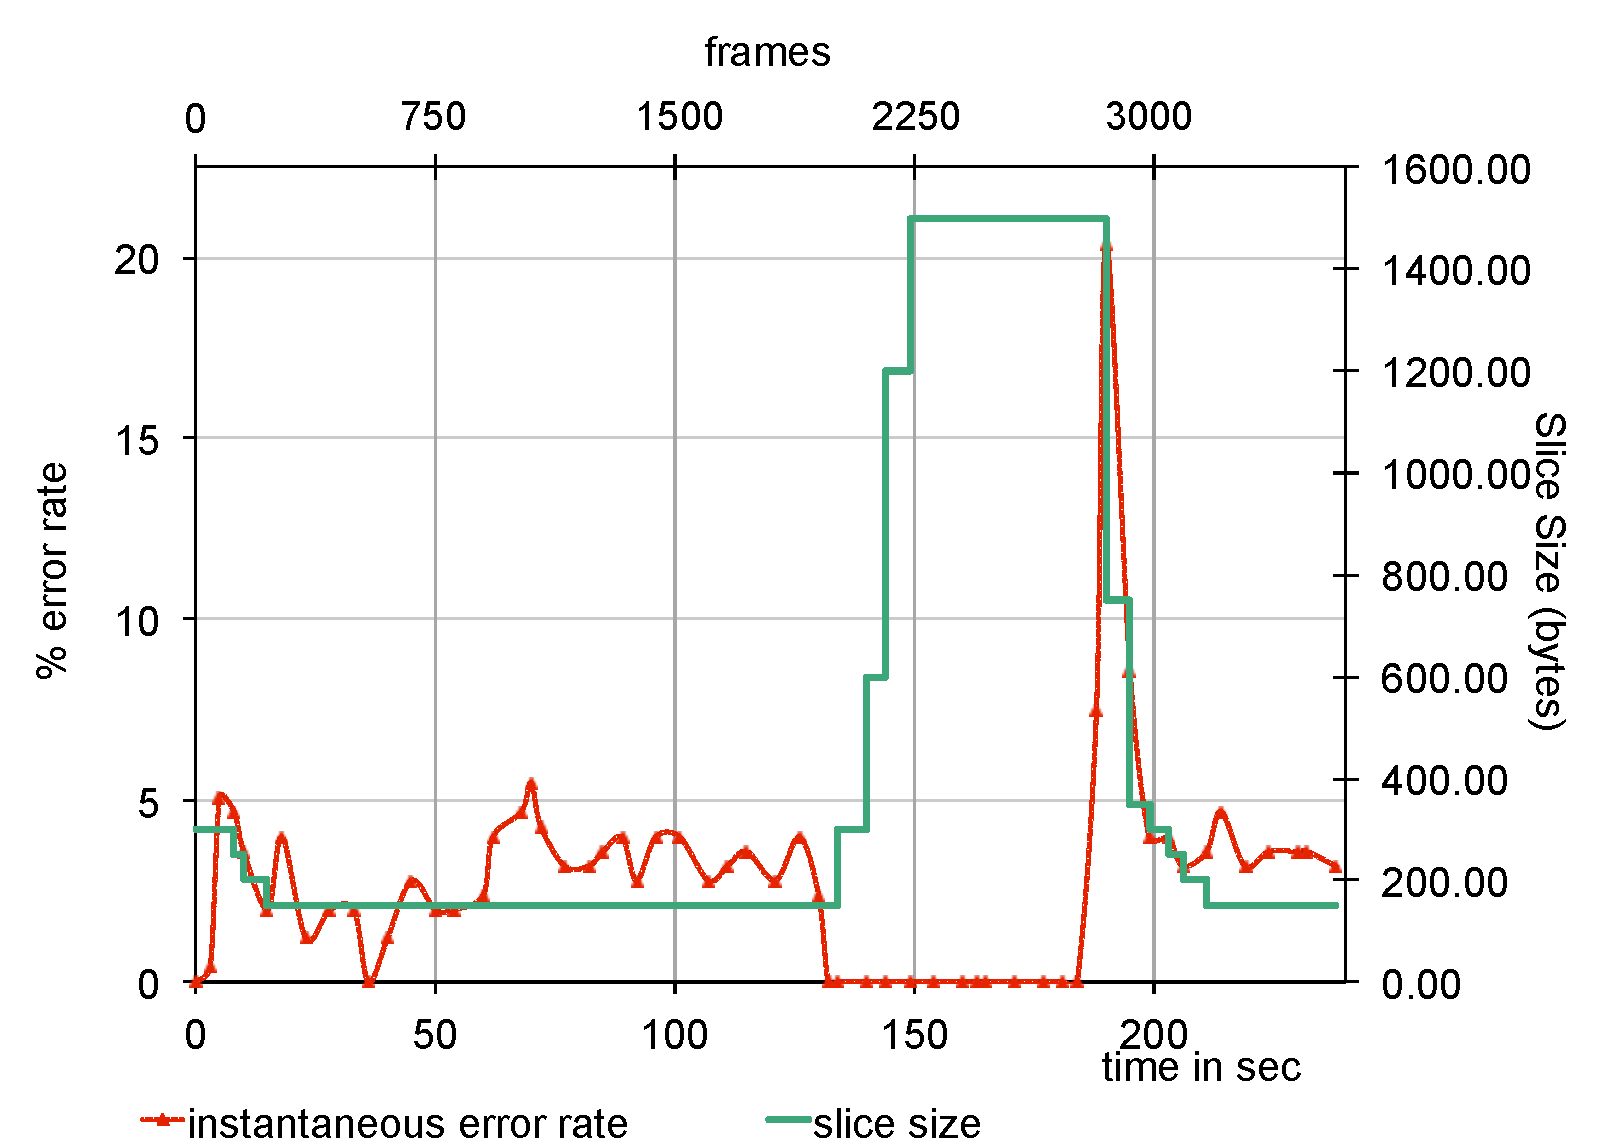
\includegraphics[width=0.9\textwidth]{chap6_ssa_adapt}
% }
% \caption{Adapting Slice Sizes due to variable error rates.}
% \label{fig:ssa_adapt}
% \end{figure}

The error-resilience mechanisms are modeled as a function of observed packet
loss and end-to-end delay. For the chosen call scenarios, the applicability of
the error-resilience mechanisms are represented in figure~\ref{fig:apply_err}.

\begin{figure}
\centerline {
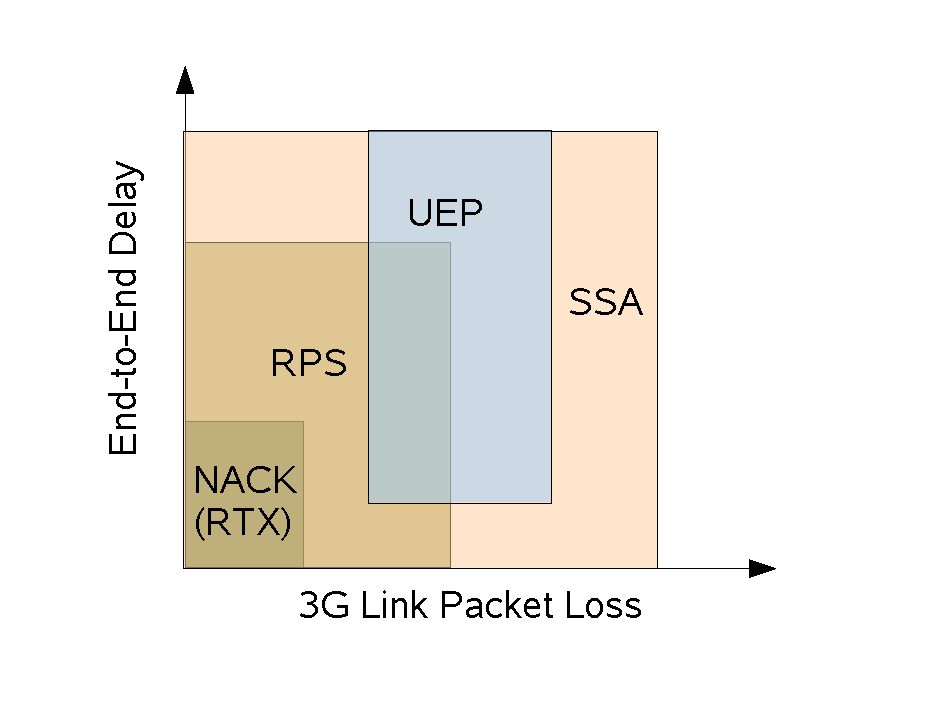
\includegraphics[width=0.9\textwidth]{chap6_apply_err}
}
\caption{Applicability of the error-resilience schemes in heterogeneous
environment containing both wireless and wired links.}
\label{fig:apply_err}
\end{figure}

\section{Using FEC for Congestion Control}

% Figure with the idea: FEC for CC

% Table of FEC, C-NADU and RRTCC :)